\documentclass[10pt, aspectratio=169, t]{beamer}

% NOTE %
% In order to compile this file as is, you'll need a few things:
%   1. mtheme (https://github.com/matze/mtheme)
%   2. Fira Sans font from Mozilla (https://www.mozilla.org/en-US/styleguide/products/firefox-os/typeface/)
% In addition, you'll need to compile using XeTeX.  If that all sounds too complicated, just change the theme below.

\usetheme{metropolis}

\usepackage{spot}
\usepackage{color}
\usepackage{booktabs}
\usepackage{makecell}

\usepackage{pgf}
\usepackage{tikz}
\usetikzlibrary{arrows,automata,shapes}
\usepackage{qrcode}

\title{New Instructor Training}
\subtitle{}

\author{{\large Jason Siefken}\\
University of Toronto\\[1cm]
\textcolor{mLightBrown}{U of T classes being 10 minutes past the hour; we will begin 10 minutes past.}\\[2cm]$^*$With materials from Professors Mayes-Tang and Gracia-saz}
\date{}

\begin{document}

\setspotlightstyle{rectangle, rounded corners,fill=structure.fg!15!white,path fading=none}

\maketitle


%
\begin{frame}{Warmup}
	Form groups of 4--5 with the restriction:
	\begin{itemize}
		\item No two group members are teaching the same F/Y course.
	\end{itemize}

	Learn about each of your group member:
	\begin{itemize}
		\item What do they research/study?
		\item What was a memorable experience they had as a TA?
	\end{itemize}
\end{frame}

\section{The 5 Principles}
\begin{frame}{The 5 Principles}
\begin{columns}
\begin{column}{0.5\textwidth}
	\begin{block}{Principles}
		\begin{enumerate}
			\item Give students time to struggle.
			\item Say yes to your students' ideas.
			\item Don't be the answer key.
			\item Motivate with questions.
			\item Play!
		\end{enumerate}
		\begin{center}
			\qrcode{https://mathforlove.com/2015/06/5-principles-of-extraordinary-math-teaching/}
		\end{center}
	\end{block}
\end{column}
\begin{column}{0.5\textwidth}  %%<--- here
	\begin{block}{Questions?}
		\begin{itemize}
			\item Think about the best instructor you ever had. Did any of the principles apply to them?
			\item Can these principles apply in a university setting?
		\end{itemize}
	\end{block}
\end{column}
\end{columns}
\end{frame}


\section{Learning Objectives}
\begin{frame}{Learning Objectives}
\begin{columns}
\begin{column}{0.5\textwidth}
	\begin{block}{Learning objectives}
		answer the questions\ldots
		\begin{itemize}
			\item What do you want students to \alert{learn} by the end of a lesson?
			\item What do you want students to be able to \alert{do} by the end of a lesson?
			\item What do you want to \alert{stick} with students at the end of a course? Several years after a course?
		\end{itemize}
	\end{block}
\end{column}
\begin{column}{0.5\textwidth}  %%<--- here
	\pause
	\begin{block}{Questions?}
		\large
		\begin{itemize}
			\item Why would you\,---\,as an instructor\,---\,want to write learning objectives before planning a lesson?
		\end{itemize}
	\end{block}
\end{column}
\end{columns}
\end{frame}

\begin{frame}{Effective Learning Objectives}
\begin{columns}
\begin{column}{0.5\textwidth}
	\begin{block}{Good learning objectives}
		\begin{itemize}
			\item Refer to \textcolor{mLightGreen}{specific skills/beliefs/attitudes} you want students to have.
			\item Are \textcolor{mLightGreen}{measurable} and provide the context in which they will be measured.\\[1.5cm]
			\item Avoid vague phrases like ``students will understand'' and ``students will see''.
		\end{itemize}
	\end{block}
\end{column}
\begin{column}{0.5\textwidth}  %%<--- here
	\metroset{block=fill}
	\begin{block}{Examples}
		\metroset{block=transparent}

		~\begin{minipage}{.95\textwidth}
			\begin{block}{By the end of the course, }

			students will be able to \alert{apply} the comparison test to determine
			whether a series of the form $\sum 1/x^\alpha$ converges when $\alpha>0$ is a fraction.
			\end{block}

			\begin{block}{By the end of this lecture,}

			students will be able to \alert{explain} how the ``square root algorithm''
			relates to Newton's method.
			\end{block}
		\end{minipage}


	\end{block}
\end{column}
\end{columns}
\end{frame}

\begin{frame}{Example Learning Objectives}


\begin{columns}
\begin{column}{0.5\textwidth}
	\metroset{block=fill}

	{\noindent
	\bfseries
	By Midterm 1, students will be able to}
	\begin{block}{(MAT137)}
		\alert{apply} the $\varepsilon$-$\delta$ definition of limit to prove
		whether a rational function has a horizontal asymptote.
	\end{block}

	\begin{block}{(MAT136)}
		\alert{determine}, using a slope field, whether a solution to an initial value problem
		has a horizontal asymptote.
	\end{block}

	\begin{block}{(MAT133)}
		\alert{produce} a real-word example of a function with a horizontal asymptote.
	\end{block}

\end{column}
\begin{column}{0.5\textwidth}  %%<--- here
	\begin{block}{Questions?}
		\begin{itemize}
			\item 
			How would class be similar/different for each of the learning objectives?
		\end{itemize}
	\end{block}
\end{column}
\end{columns}
\end{frame}


\begin{frame}{Dee Fink's Framework}
	\vspace{-.5cm}
\begin{columns}
\begin{column}{0.5\textwidth}
	\begin{block}{Situational Factors}
		\begin{enumerate}
			\item \alert{Class Context}: Number of students? Upper division/lower division?
				Hours of class per week? Tutorials?
			
			\item \alert{External Context}: Restrictions from the University? Department? Society?

			\item \alert{Subject}: Theoretical? Applied? Actively researched?
			
			\item \alert{Learners}: What are the goals of the learners? What is their life situation?

			\item \alert{Teacher}: What are your teaching strengths? Expertise?

			
		\end{enumerate}
	\end{block}
\end{column}
\begin{column}{0.5\textwidth}  %%<--- here
	\begin{block}{Types of Goals}
		\begin{itemize}
			\item \alert{Foundational}: What information/ideas are important to \textbf{understand and remember}? 
			\item \alert{Application}: What thinking/skills should a student \textbf{acquire}? 
			\item \alert{Integration}: What ideas should students \textbf{connect} with their other courses/profession/life?
			\item \alert{Human}: How should students \textbf{interact} with each other? Themselves? How should they \textbf{feel}? 
			\item \alert{Meta}: Learning how to learn. 
		\end{itemize}
	\end{block}
\end{column}
\end{columns}
\end{frame}



\begin{frame}{Activity}
	\textcolor{mLightGreen}{\textbf{Review your mini-lecture. What are its learning objectives?}}

	\vspace{-.5cm}
\begin{columns}
\begin{column}{0.5\textwidth}
	\begin{block}{Situational Factors}
		\begin{enumerate}
			\item \alert{Class Context}: Number of students? Upper division/lower division?
				Hours of class per week? Tutorials?
			
			\item \alert{External Context}: Restrictions from the University? Department? Society?

			\item \alert{Subject}: Theoretical? Applied? Actively researched?
			
			\item \alert{Learners}: What are the goals of the learners? What is their life situation?

			\item \alert{Teacher}: What are your teaching strengths? Expertise?

			
		\end{enumerate}
	\end{block}
\end{column}
\begin{column}{0.5\textwidth}  %%<--- here
	\begin{block}{Types of Goals}
		\begin{itemize}
			\item \alert{Foundational}: What information/ideas are important to \textbf{understand and remember}? 
			\item \alert{Application}: What thinking/skills should a student \textbf{acquire}? 
			\item \alert{Integration}: What ideas should students \textbf{connect} with their other courses/profession/life?
			\item \alert{Human}: How should students \textbf{interact} with each other? Themselves? How should they \textbf{feel}? 
			\item \alert{Meta}: Learning how to learn. 
		\end{itemize}
	\end{block}
\end{column}
\end{columns}
\end{frame}

\section{Mini-lectures}

\section{Lesson Planning}
\begin{frame}{Lesson Planning---Objectives}

	{By the end of today you will be able to}
	\begin{itemize}
		\item \alert{write} applicable \textcolor{mLightGreen}{learning goals} for a lesson in your course;
		\item \alert{create} a \textcolor{mLightGreen}{lesson plan} based on your learning goals (``Backwards Design'');
		\item \alert{describe} at least one \textcolor{mLightGreen}{activity} that can tighten the ``learning cycle''.
	\end{itemize}

\end{frame}

\begin{frame}{Lesson Planning}

	{\Large Lesson plans are documents that outline}
	\begin{itemize}
		\item \alert{what} you will do in your class and
		\item \alert{when} it will happen.
	\end{itemize}

	\pause
	\bigskip
	{\Large Backwards Design}

	Design happens in three stages by identifying

		\tikzstyle{block} = [rectangle, fill=mLightGreen, text=white,
		    text width=3.3cm, text centered, rounded corners, minimum height=2.3cm, outer sep=7pt]
		    
		    \vfill
		\begin{tikzpicture}[node distance = 5cm, auto]
		    % Place nodes
			\node (init) [block] {\begin{minipage}{3cm}\bfseries What do you want students to know?\end{minipage}};
		    \node (f) [block, right of=init] {\begin{minipage}{3cm}\bfseries How could you measure this knowledge?\end{minipage}};
		    \node (g) [block, right of=f] {\begin{minipage}{3cm}\bfseries What will you and the students be doing during class?\end{minipage}};
		    % Draw edges
		    \path [->, very thick, color=mLightGreen] (init.east) edge [bend left=20] (f.west);
		    \path [->, very thick, color=mLightGreen] (f.east) edge [bend left=20] (g.west);
			%\path [->, very thick] (f.west) edge [bend left=60] (init.west);
		\end{tikzpicture}
\end{frame}

\begin{frame}{Lesson Planning}

\begin{columns}
\begin{column}{0.5\textwidth}
	Which learning goal is best for a first-year calculus course for students majoring in biology?

	\bigskip
	\begin{block}{By the end of the course, students should be able to\ldots
		}
	\begin{enumerate}
		\item[(A)] Explain why the graph of an antiderivative is the shape that it is.
		\item[(B)] Graph antiderivatives.
		\item[(C)] Given the graph of a function, sketch an antiderivative passing through a particular point.
		\item[(D)] Understand antiderivatives and the FTC.
	\end{enumerate}
	\end{block}
\end{column}
\begin{column}{0.5\textwidth}  %%<--- here
	\pause
	\large
	\begin{itemize}
		\item How could you \alert{measure} (C)?
		
		\pause

		\item What could you \alert{do in class} to achieve (C)?
	\end{itemize}
\end{column}
\end{columns}
\end{frame}




%% ----------------------------------------------------------------------

\section{The Learning Cycle}

%% ----------------------------------------------------------------------  

\begin{frame}{The Learning Cycle}


	\begin{center}
{\Large Simplified model of learning}

		\tikzstyle{block} = [rectangle, draw, fill=blue!20, 
		    text width=10em, text centered, rounded corners, minimum height=4em, outer sep=3pt]
		    
		    \vfill
		\begin{tikzpicture}[node distance = 2cm, auto]
		    % Place nodes
		    \node [block] (init) {\Large Practice};
		    \node [block, below of=init] (f) {\Large Feedback};
		    % Draw edges
			\path [->, very thick] (init.east) edge [bend left=60] (f.east);
			\path [->, very thick] (f.west) edge [bend left=60] (init.west);
		\end{tikzpicture}
		\vfill
	\end{center}
\end{frame}



\begin{frame}{The Learning Cycle}

\vspace{3em}

\begin{block}{}
	Students need to
\vspace{-.5em}
	\begin{itemize}
		\item \alert{know \emph{what}} to practice
		\item be \alert{motivated}
		\item be able to \alert{judge improvements}/regressions
		\item be \alert{comfortable} making mistakes
		\item[] ~~~~~~~~~~~~~~~~~~~~~~~~~~~~~~~\vdots
	\end{itemize}
\end{block}

\end{frame}

\begin{frame}{Identify where \emph{Practice} and \emph{Feedback} occur}

\begin{columns}
\begin{column}{0.5\textwidth}
	\begin{block}{``Lecture-based'' Analysis Class}
		\begin{itemize}
			\item Background

			\item Definition
				\begin{itemize}
			\item Easy example
			\item Hard example
				\end{itemize}
			\item Theorem
			\item Proof
				\begin{itemize}
			\item Outline
			\item Details
			\item Re-emphasis of important/hard idea
				\end{itemize}
			
			\item[] ~~~~~~~~~~\vdots
			\item Homework
		\end{itemize}
	\end{block}
\end{column}
\begin{column}{0.5\textwidth}  %%<--- here
	\begin{block}{``Active'' Calculus Class}
		\begin{itemize}
			\item Background
			\item Ask a ``hard'' question
			\item Definition
				\begin{itemize}
			\item Have students generate examples
			\item Discuss examples
				\end{itemize}
			\item Re-ask similar question
				\begin{itemize}
			\item Get student ideas
			\item Explain relation to definition
				\end{itemize}
			\item[] ~~~~~~~~~~\vdots
			\item Homework
		\end{itemize}
	\end{block}
\end{column}
\end{columns}
\end{frame}

%% ----------------------------------------------------------------------

\section{Techniques to Tighten the Loop}

%% ----------------------------------------------------------------------

\begin{frame}{Think, Pair Share \& Friends}

	\vfill
	\metroset{block=fill}

	\begin{block}{\Large Think, Pair-Share}
		\Large
		\begin{itemize}
			\item Ask question
			\item Individual thinking (\& voting)
			\item Pair discussion (\& voting)
			\item Class discussion
		\end{itemize}
	\end{block}

\end{frame}



\begin{frame}{Think, Pair Share Example}
	\begin{columns}
	\begin{column}{0.7\textwidth}

		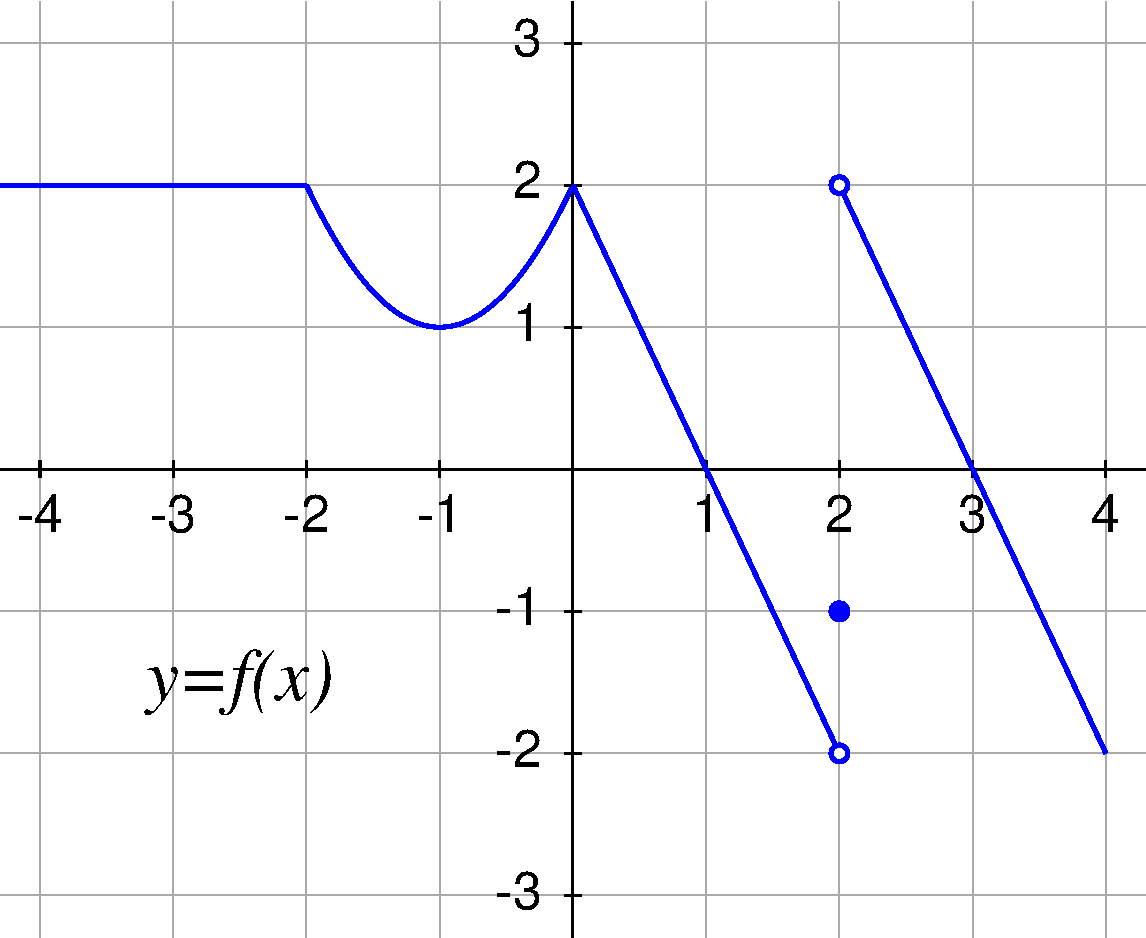
\includegraphics[width=.9\textwidth]{think-pair-share-graph.pdf}

	\end{column}
	\begin{column}{0.3\textwidth}  %%<--- here
		\begin{block}{Compute}
			\begin{enumerate}
				%\item {\Large $\displaystyle \lim_{x\to 2} f(x)$}
				\item {\Large $\displaystyle \lim_{x\to 0} f(f(x))$}
			\end{enumerate}
		\end{block}
		\pause
		\begin{block}{Choose from}
			\begin{itemize}
				\item[] $-2$
				\item[] $-1$
				\item[] $2$
				\item[] DNE
				\item[] other
			\end{itemize}
		\end{block}
	\end{column}
	\end{columns}
\end{frame}

\begin{frame}{Think, Pair Share Example}
		\begin{block}{}
			\Large
			Which of these is a correct description of the set $E$ of even integers?
			\begin{enumerate}
				\item $\displaystyle E=\{n\in \mathbb Z:\forall\, a\in\mathbb Z,\ n=2a\}$
				\item $\displaystyle E=\{n\in \mathbb Z:\exists\, a\in\mathbb Z\ \text{s.t.}\ n=2a\}$
			\end{enumerate}
		\end{block}
		\pause
		\begin{block}{}
			\Large
			For $n=4$, which of the following statements is true?
			\begin{enumerate}
				\item[3.] $\forall\, a\in\mathbb Z,\ n=2a$
				\item[4.] $\exists\, a\in\mathbb Z\ \text{s.t.}\ n=2a$
			\end{enumerate}
		\end{block}
\end{frame}

\begin{frame}{Guided Exercise Example}
			\Large
			The function $\coth$, defined by
			\alert{\[
				\coth x=\frac{e^{2x}+1}{e^{2x}-1},
			\]}
			is called the ``hyperbolic cotangent''.
			\begin{enumerate}
				\item Find its domain.
				\item Find its \alert{three} asymptotes.
				\item To save you time, I have computed that $\coth'$ is
always negative (on its domain). With this
information, sketch the graph of $\coth$.
			\end{enumerate}
\end{frame}

%% ----------------------------------------------------------------------
\section{Making Good Questions}

\begin{frame}{Making Good Questions}

\vspace{3em}

	A good questions ties to your learning goals and
	\begin{itemize}
		\item re-enforces, generates the need for, or explores a concept
		\item informs the instructor (answers will indicate whether to move on)
		\item is scaffolded (chunked)
		\item can be reasonably solved (in 1--4 minutes)
		\item generates controversy (depending on your goals)
	\end{itemize}

\end{frame}

\section{Lesson Planning Pitfalls}
\begin{frame}{The Content Issue}

	\begin{center}
	{\Large How do I cover it all?}
	\end{center}

	\pause
	\begin{itemize}
		\item \textcolor{mLightGreen}{Prioritize learning goals}
			\begin{itemize}
				\item Is surface-level understand of many things important? (i.e., coverage)
				\item Is deep understanding of \emph{some} thing important?
				\item What will help the students as future learners?
				\item Which goals will have a lasting impact? (e.g., past the midterm)
			\end{itemize}
		\item \textcolor{mLightGreen}{You don't need to ``say it in class'' for students to learn it}
			\begin{itemize}
				\item What goals are best addressed in homework? Through readings?
				\item What goals are easiest for the students to achieve themselves? (i.e.,
					without a subject-matter expert present)
			\end{itemize}
		\item \textcolor{mLightGreen}{Discuss with other instructors}
			
	\end{itemize}
\end{frame}

\section{Make a Lesson Plan}
\begin{frame}{Make a Lesson Plan}

	Resources available at\\ \url{https://github.com/siefkenj/teaching-resources}
	\begin{center}
		\qrcode[height=1.5in]{https://github.com/siefkenj/teaching-resources}
	\end{center}
\end{frame}

\section{Instructor Panel}

\end{document}
